% !TeX spellcheck = en_GB
\documentclass[a4paper, 10pt]{article}
\usepackage{pgf}
\usepackage{eurosym}
\usepackage{graphicx}
\usepackage{wasysym}
\usepackage{hyperref}
\usepackage{listings}
\usepackage{pxfonts}
\usepackage{verbatim}
\usepackage{color}
\usepackage{xcolor}
\usepackage{wrapfig}
\usepackage{enumitem}
\usepackage{booktabs}
\usepackage{tabularx}

\hypersetup{
    bookmarks=true,         % show bookmarks bar?
    unicode=true,          % non-Latin characters in Acrobat’s bookmarks
    pdftoolbar=true,        % show Acrobat’s toolbar?
    pdfmenubar=true,        % show Acrobat’s menu?
    pdffitwindow=true,     % window fit to page when opened
    pdftitle={Assignment 2},    % title
    pdfauthor={Paul Vesey},     % author
    pdfsubject={Construction Project Management},   % subject of the document
    pdfcreator={},   % creator of the document
    pdfproducer={xelatex}, % producer of the document
    pdfkeywords={'Project Management' }, % list of keywords
    pdfnewwindow=true,      % links in new PDF window
    colorlinks=true,       % false: boxed links; true: colored links
    linkcolor=violet,          % color of internal links (change box color with linkbordercolor)
    citecolor=magenta,        % color of links to bibliography
    filecolor=red,      % color of file links
    urlcolor=blue           % color of external links
}

\setlength\parindent{0pt}
\begin{document}

\lstset{language=HTML,
				basicstyle=\small,
				breaklines=true,
        numbers=left,
        numberstyle=\tiny,
        showstringspaces=false,
        aboveskip=-20pt,
        frame=leftline
        }
				
\begin{table}%
	\begin{minipage}{0.4\textwidth}%
			
\includegraphics[width=1\textwidth]{./img/LITlogo.jpg}
	\end{minipage}
	\qquad
	\centering
	\parbox{0.4\textwidth}{
		\begin{large}			
			\begin{tabular}{| r | l |} \hline
				Subject: & \textbf{Construction Project Management}\\
				Course: & \textbf{CPM Special Purpose Award}\\	
				Session: & \textbf{Autumn 2020}\\
				Lecturer: & \textbf{Paul Vesey \footnotesize{BEng, MIE, HDip}}\\
				\hline
			\end{tabular}
		\end{large}			
	}
\end{table}
\vspace{0.25cm}	


\part*{Assignment 3 (30\%)- Earned Value Tracking in Microsoft Project}



\begin{tabularx}{\textwidth}{ |X|X| }
	\hline
	\textbf{Issue Date:} & As stated on Microsoft Teams \\
	\hline 
	\textbf{Submission Date:}  & As stated on Microsoft Teams  \\
	\hline
\end{tabularx}

\section*{Introduction}

In this assignment you are going to implement EVM a simple Microsoft Project Plan.  The key deliverables for this project are:

\begin{enumerate}
	\item Microsoft Project Project Plan, updated with a Baseline and EVM information
	\item Screenshots of the Status Dates, placed into an MS Word document
\end{enumerate}




\section*{Scenario}

You have been provided with a Microsoft Project file for the construction of a domestic dwelling.  This file is based on the sample file provided by Microsoft.  The .mpp file contains a simple Gantt chart, resources allocations including associated costs. \\

The objective of the assignment is to create EVM data for the status dates indicated in Table \ref{tab:StatusDates}.  Details of the columns necessary are provided in Figure \ref{fig:TableData}.  You will need to add some of the columns manually.  Please note that 'Actual Cost' and 'Actual Finish' columns are necessary to edit the data generated by Microsoft Project.  You will also need to set a 'Baseline' for the EVM data to be activated.\\

As part of this assignment you are required to edit the 'Actual Cost' and 'Actual Finish' columns in order to generate variances from the planned data.  This is to provide you with experience of tracking project performance within the tool.  You are free to set the Actual Costs or Actual Finish dates as you see fit. 

\begin{table}
	\centering

	\begin{tabular}{ |c|r| }
		\hline
		\textbf{No.} & \textbf{Status Date} \\
		\hline 
		1 &  9 Dec 2020\\ 
		2 &  1 Feb 2021 \\ 
		3 &  1 Apr 2021\\ 
		4 &  1 Jun 2021 \\
		\hline
	\end{tabular}
	\caption{Status Dates}	
	\label{tab:StatusDates}
\end{table}


\section*{Submission}
Your completed assignment comprising all computer files are to be uploaded to Microsoft Teams on or before the date and time indicated.  Key components of the submission are:
\begin{itemize}
	\item Microsoft Project (.mpp) file
	\item Microsoft Word (.docx) file containing screenshots
\end{itemize}



\subsection*{Marking Scheme}

\begin{table}[h!]
     \begin{center}
     \begin{tabular}{p{5cm}  p{5cm} }
     \toprule
      \textbf\large{Element} & \textbf\large{Proportion} \\ 
    \cmidrule(r){1-1}\cmidrule(lr){2-2}
      \textbf{Microsoft Project File} & \textbf{80\%}\\
      \textbf{Microsoft Word File} & \textbf{20\%}
      
      \\ \bottomrule
      \end{tabular}
      \label{tbl:markSchemeAsmt3}
      \end{center}
 \end{table}

\newpage

\begin{sidewaysfigure}
	\centering
	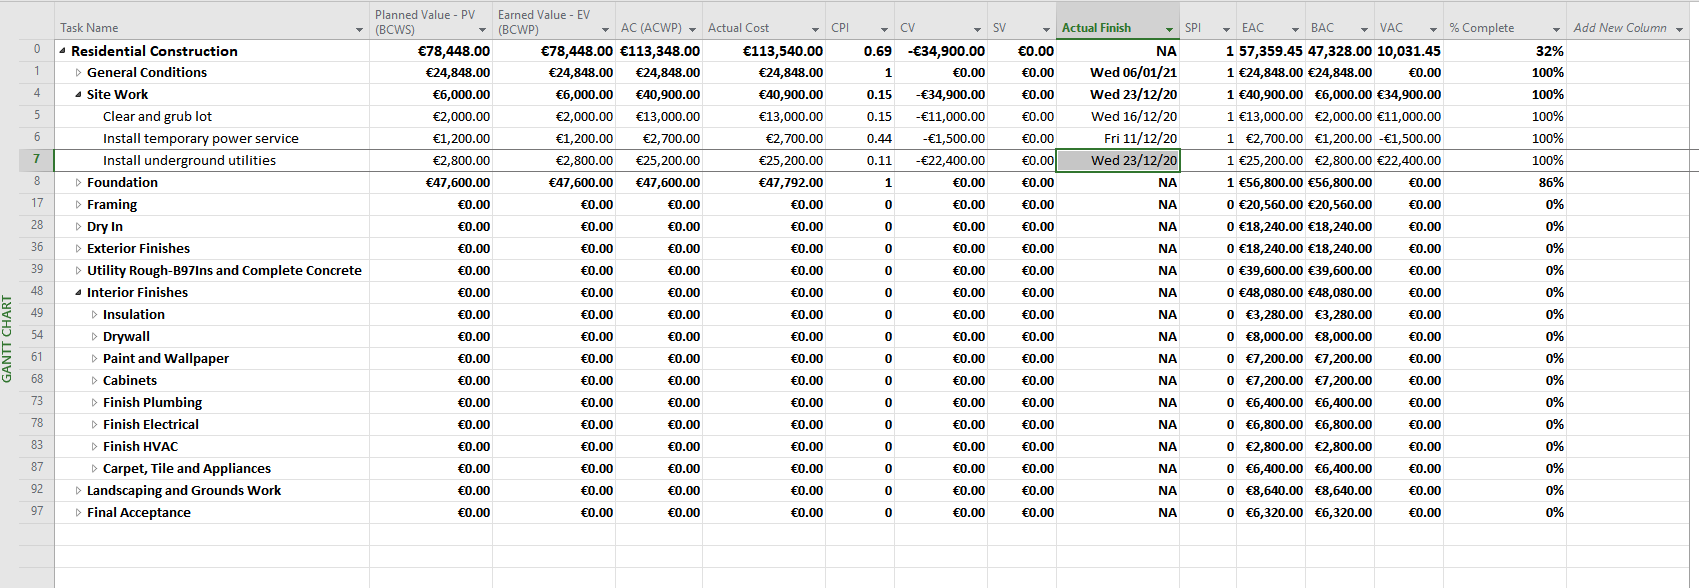
\includegraphics[width=1.0\linewidth]{./img/TableConfiguration.png}
	\caption{Sample EVM Data}
	\label{fig:TableData}
\end{sidewaysfigure}

\end{document}